%%%%%%%%%%%%%%%%%%%%%%%%%%%%%%%%%%%%%%%%%%%%%%%%%%%%%%%%%%%%%%%%%%%%%%%%%%%%%
%
%  System        : 
%  Module        : 
%  Object Name   : $RCSfile$
%  Revision      : $Revision$
%  Date          : $Date$
%  Author        : $Author$
%  Created By    : Robert Heller
%  Created       : Wed May 31 20:05:00 2017
%  Last Modified : <171104.0937>
%
%  Description 
%
%  Notes
%
%  History
% 
%%%%%%%%%%%%%%%%%%%%%%%%%%%%%%%%%%%%%%%%%%%%%%%%%%%%%%%%%%%%%%%%%%%%%%%%%%%%%
%
%    Copyright (C) 2017  Robert Heller D/B/A Deepwoods Software
%			51 Locke Hill Road
%			Wendell, MA 01379-9728
%
%    This program is free software; you can redistribute it and/or modify
%    it under the terms of the GNU General Public License as published by
%    the Free Software Foundation; either version 2 of the License, or
%    (at your option) any later version.
%
%    This program is distributed in the hope that it will be useful,
%    but WITHOUT ANY WARRANTY; without even the implied warranty of
%    MERCHANTABILITY or FITNESS FOR A PARTICULAR PURPOSE.  See the
%    GNU General Public License for more details.
%
%    You should have received a copy of the GNU General Public License
%    along with this program; if not, write to the Free Software
%    Foundation, Inc., 675 Mass Ave, Cambridge, MA 02139, USA.
%
% 
%
%%%%%%%%%%%%%%%%%%%%%%%%%%%%%%%%%%%%%%%%%%%%%%%%%%%%%%%%%%%%%%%%%%%%%%%%%%%%%

\chapter{SMCSenseHAT: Stall Motor Control and Sense HAT}

This is a circuit board to for an add-on board for a Raspberry Pi B+ that will
control  two  stall-motor  turnout  motors for a model  railroad.  It also has
sense  logic to return the state of the  turnouts,  using one pole of the DPDT
contacts in the stall-motor (typical of Tortoise stall-motors).

The circuit board uses a 40pin header socket to connect to the 40pin header on
the  Raspberry Pi B+ and can use a  stack-through  header to allow  additional
boards to be stacked on top of it.

The circuit board presented in the SMCSenseHAT1 directory is nearly identical 
to this one.  The only difference is the use of a different set of four GPIO 
pins.


\section{GPIO Pins Used and stacking restrictions.}

This board uses four GPIO pins:

\begin{description}
\item[WiringPi 0, BCM 17] Motor Select 1: select the position of stall motor 
1. 
\item[WiringPi 1, BCM 18] Motor Select 2: select the position of stall motor 
2. 
\item[WiringPi 2, BCM 27] Point Sense 1: return the state of the points for 
stall motor 1. 
\item[WiringPi 3, BCM 22] Point Sense 2: return the state of the points for 
stall motor 2. 
\end{description}

Each of the motor drive circuits is through a transistor that can handle 1 amp 
continuous collector current, which is way more needed to drive typical stall 
motor.  It is enough to drive a pair of stall motors, wired in parallel as 
would be the case for a cross over.

Because this board is hardwired to use four specific GPIO pins it is not 
possible to use two or more of these boards on given Raspberry Pi.  But in the 
SMCSenseHAT1 directory is a nearly identical board, that uses a different set 
of four GPIO pins:

\begin{description}
\item[WiringPi 4, BCM 23] Motor Select 1: select the position of stall motor 
1. 
\item[WiringPi 5, BCM 24] Motor Select 2: select the position of stall motor 
2. 
\item[WiringPi 6, BCM 25] Point Sense 1: return the state of the points for 
stall motor 1. 
\item[WiringPi 7, BCM 4] Point Sense 2: return the state of the points for 
stall motor 2. 
\end{description}

It is possible use one each of the SMCSenseHAT and SMCSenseHAT1 boards to 
handle four separate turnouts.  You should only connect at most one of each of 
these boards on a single Raspberry Pi.

\section{Circuit Description}

\begin{figure}[hbpt]\begin{centering}%
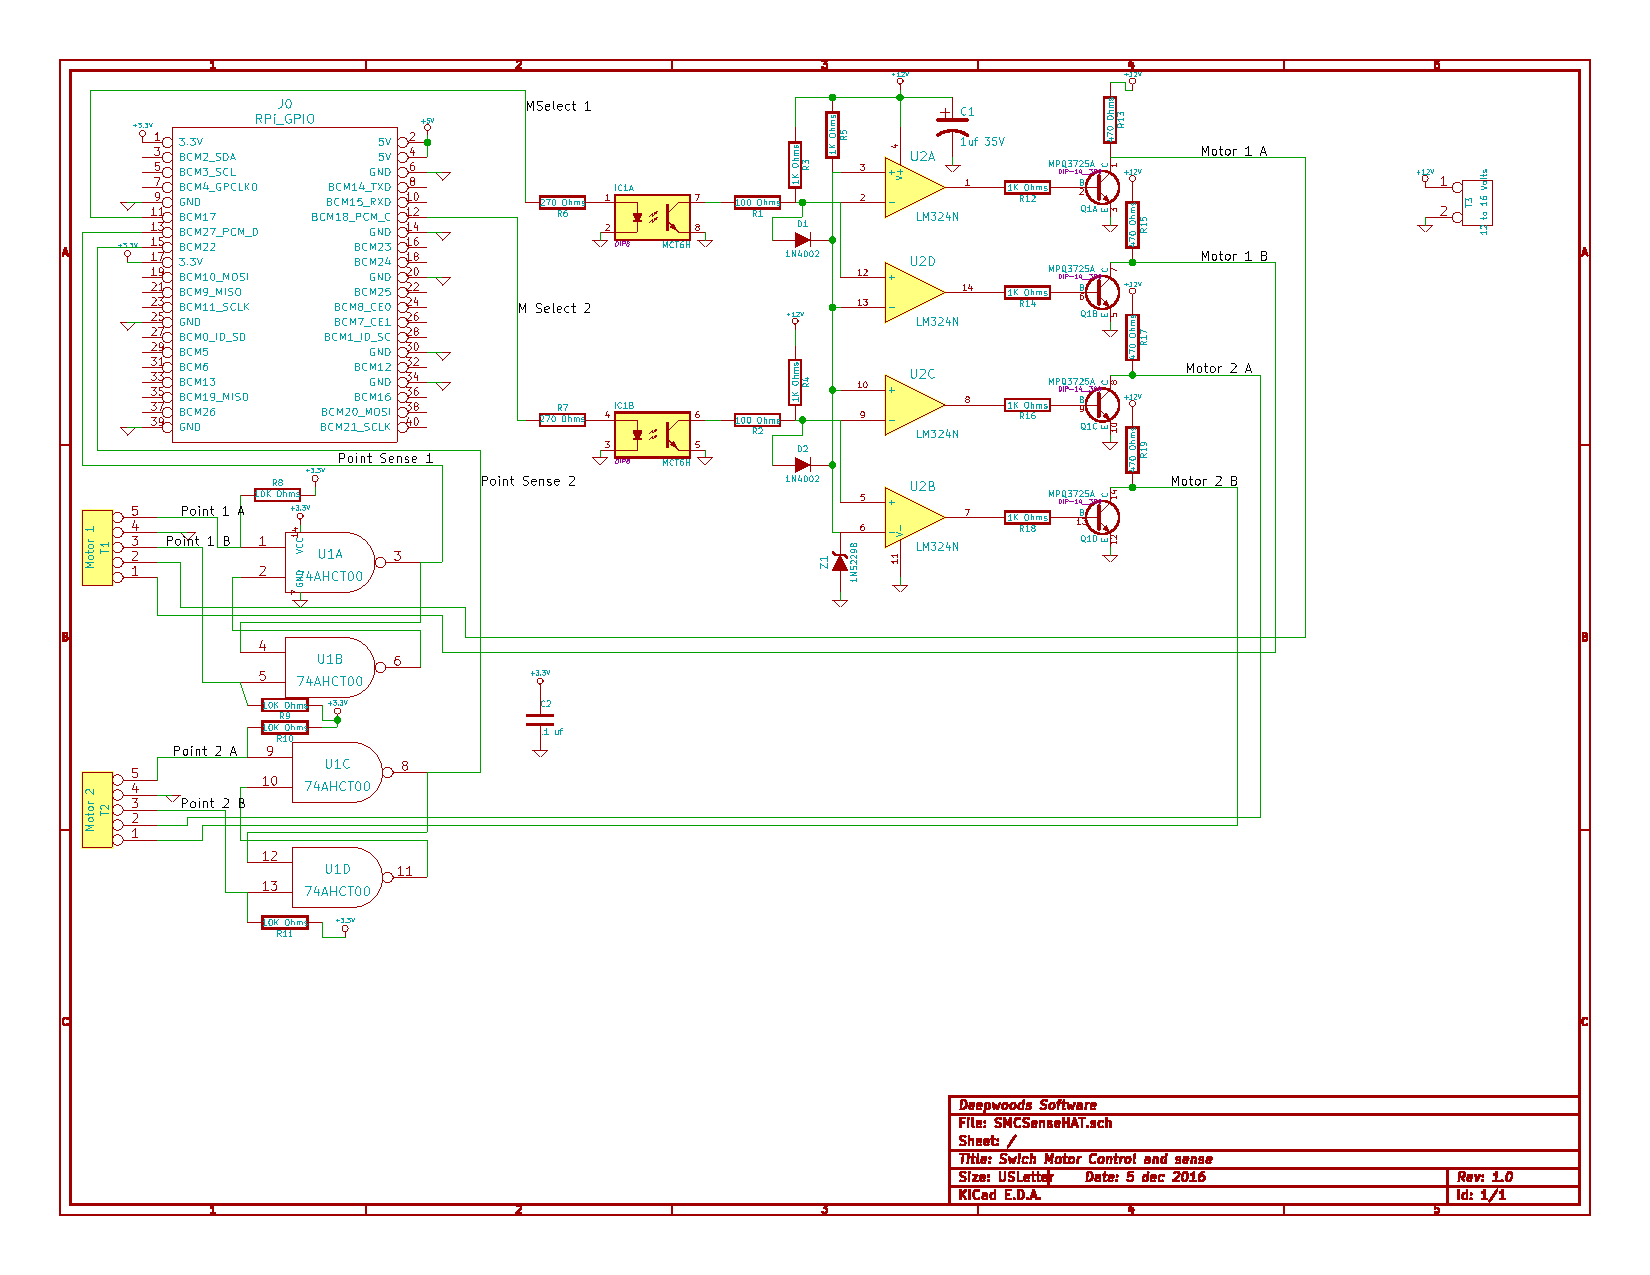
\includegraphics[width=5in]{SMCSenseHAT.pdf}
\caption{Circuit Diagram of the SMCSenseHAT}
\end{centering}\end{figure}
This circuit contains two sections.  There is an output section that contains 
a dual opto-isolator, a quad op-amp, and a quad driver (NPN) transistor.  An 
opto-isolated GPIO output pin drives one pair of op-amps, which in turn drive 
a pair of driver transistors.  Each GPIO output pin drives its pair of op-amps 
on their opposite plus and minus inputs, thus driving only one or the other of 
this pair of op-amps at a time.  That is the GPIO output pin drives one op-amp 
on when the GPIO output pin is high and drives the other op-amp on when the 
GPIO output pin is low.  On the output side only one of the pair of driver 
transistors is on at a time.  This results in only one or the other of the 
motor drive connections at ground (-) and the other pulled up to 12-16 Volts 
(+).  This causes the stall motor to rotate in one or the other direction, 
moving the turnout points one way or the other.

The other section is a pair of flip-flop debounce circuits, one for each of 
two SPDT switch contacts that report the position of the turnout points.  The 
output of these flip-flops goes to a pair of GPIO input pins.

\section{Parts List}

\begin{table}[htdp]
\begin{centering}\begin{tabular}{|l|l|p{1in}|l|p{.5in}|}
\hline
Value&Qty&Refs&Mouser Part Number&Adafruit Part Number \\
\hline
1uf 35V&1&C1&74-199D105X9035A1VE3& \\
\hline
.1 uf&1&C2&21RZ310-RC& \\
\hline
1N4002&2&D1 D2&833-1N4002-TP& \\
\hline
MCT6H&1&IC1&782-MCT6H& \\
\hline
RPi GPIO Header&1&J0&855-M20-6102045&2223 \\
\hline
MPQ3725A&1&Q1&610-MPQ3725A& \\
\hline
100 Ohms&2&R1 R2&603-CFR-25JR-52100R& \\
\hline
470 Ohms&4&R13 R15 R17 R19&279-CFR50J470R& \\
\hline
1K Ohms&7&R3 R4 R5 R12 R14 R16 R18&279-2-1623927-3& \\
\hline
270 Ohms&2&R6 R7&603-CFR-25JR-52-270R& \\
\hline
10K Ohms&4&R8 R9 R10 R11&603-CFR-25JR-5210K& \\
\hline
Motor terminals&2&T1 T2&571-282834-5& \\
\hline
12 to 16 Volts terminals&1&T3&571-282834-2& \\
\hline
74AHCT00&1&U1&595-SN74AHC00N& \\
\hline
LM324N&1&U2&512-LM324N& \\
\hline
1N5229B&1&Z1&512-1N5229BTR& \\
\hline
\end{tabular}
\caption{Parts list for SMCSenseHAT or SMCSenseHAT1 boards.}
\end{centering}\end{table}\footnote{Mouser Project link: 
\url{http://www.mouser.com/ProjectManager/ProjectDetail.aspx?AccessID=259711af97}.}


The only parts that might be substituted are J0 (the RPi GPIO Header), and T1 
and T2 (the Motor terminals) and T3 (the 12 to 16 Volts terminals).  The parts 
listed are for the stacking headers for the RPi GPIO Header, and screw 
terminals for the Motor terminals and the motor power terminals.  Feel free to 
select a non-stacking header for the RPi GPIO Header and to select either pin 
arrays or spring terminals for the T1, T2, and T3.


\section{Circuit Board Layout}

\begin{figure}[hbpt]\begin{centering}%
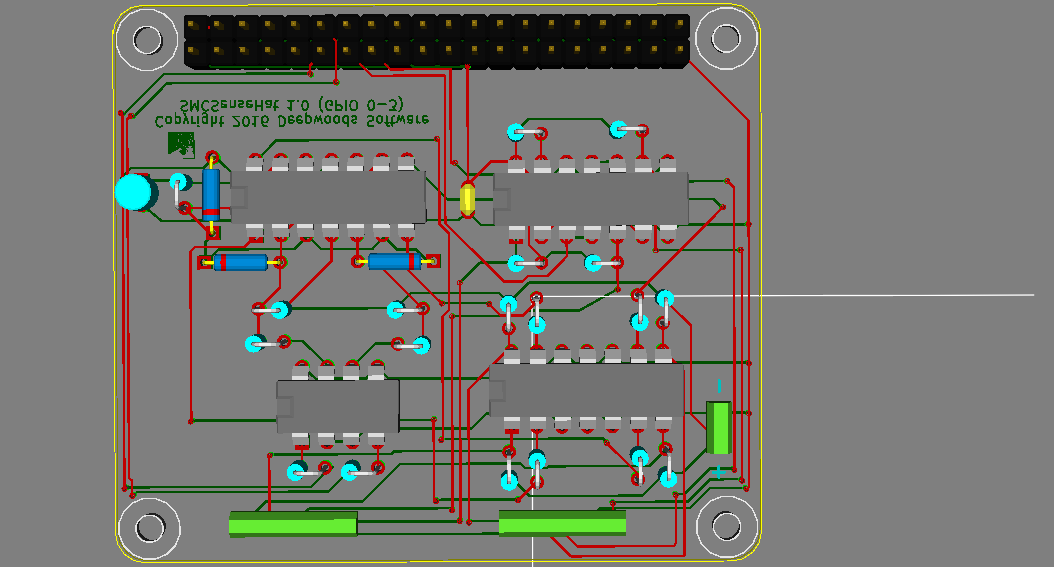
\includegraphics[width=5in]{SMCSenseHAT3DTop.png}
\caption{3D rendering of the SMCSenseHAT board}
\end{centering}\end{figure}
\begin{figure}[hbpt]\begin{centering}%
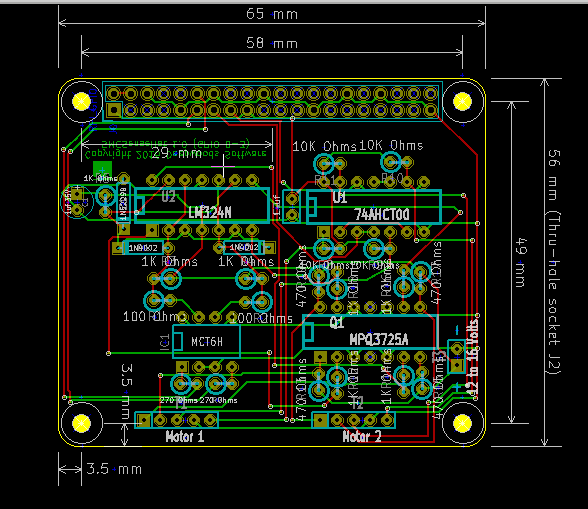
\includegraphics[width=5in]{SMCSenseHAT.png}
\caption{Fabrication image of the SMCSenseHAT board}
\end{centering}\end{figure}
Board assembly is straight forward.  You need to be careful orienting the ICs, 
diodes, and the electrolytic capacitor\footnote{The first batch of the boards 
I ordered used the wrong PCB modules for the terminals and the holes are too 
small for the screw terminal pins to go all the way in.  They can be 
``jammed'' in enough to be soldered. Pin arrays fit a little better, but still 
need some effort to seat.  The next batch I order will not have this 
problem.}. 

\section{Downloadables and Software Support}

Full design information is available on GitHub here: 
\url{https://github.com/RobertPHeller/RPi-RRCircuits/tree/master/SMCSenseHAT} 
and here:
\url{https://github.com/RobertPHeller/RPi-RRCircuits/tree/master/SMCSenseHAT1}.

This board is supported by the Model Railroad System\footnote{Available as a 
free download from Deepwoods Software at this web address: 
\url{http://www.deepsoft.com/home/products/modelrailroadsystem/}.}
\texttt{OpenLCB\_PiGPIO} daemon. A basic XML file for it is included in its
GitHub folder.

